\chapter{Servicios en móviles}\label{chap:7}
\section{Introducción al consumo de servicios desde móviles}

Esta sesión sirve de introducción al desarrollo de aplicaciones Android
utilizando Android Studio en Java.

En esta sesión se desarrolla una aplicación capaz de convertir euros
a dólares y viceversa.

Incialmente, se desarrolla un conversor simple que tiene el ratio de
conversión fijado en el código.
Posteriormente, se mejorará la aplicación utilizando una petición HTTP
que obtenga el ratio actualizado al momento.

\subsection{Converter simple}

Al crear el proyecto, seleccionamos el Android SDK Platform 33.

Posteriormente, creamos un dispositivo virtual que permita probar la
aplicación sin utilizar nuestro dispositivo físico.
Seleccionamos un Nexus 5X con Nougat (Android 7.0).

La interfaz de usuario consiste en dos campos de texto y dos botones.
Uno de los campos de texto contiene el valor en euros
y el otro la misma cantidad en dólares.
Al utilizar los botones se escribe en el otro campo de texto la cantidad
correspondiente en la moneda correspondiente.

Esto es, si se escribe el campo de texto de los euros
y se pulsa el botón de convertir a dólares,
se leerá la cantidad de euros del campo de texto de euros
y se escribirá la cantidad equivalente en dólares en el campo correspondiente.

La lógica de esta aplicación consiste en 3 funciones.

\begin{itemize}
    \item Función para convertir monedas en función de un ratio.
    \item Función para convertir de euros a dólares.
    \item Función para convertir de dólares a euros.
\end{itemize}

Por el momento se selecciona un valor fijo del ratio entre euros y dólares.

\subsection{Converter avanzado}

A continuación, se utilizará una API HTTP para obtener el ratio de euros a dólares.

Para acceder a esta API, se utilizará la libería Volley.
Para añadir Volley, utilizamos el manifiesto.

La API a utilizar (ExchangeRate) requiere que nos registremos y obtengamos un token
que nos permitirá realizar una cantidad fija de conversiones de forma gratuita.
Tras obtener dicho token, podemos introducirlo en la petición GET que realizamos con
Volley para obtener el ratio de conversión entre euros y dólares.

La petición de Volley no es instantánea, por lo que utilizamos una función de callback
que se ejecutará cuando llegue la respuesta a la petición de vuelta.
En esta función, extraemos de la respuesta el ratio de conversión y lo almacenamos
para poder utilizarlo en la función que convierte una moneda en otra.

Aquí se muestra un mensaje con el valor obtenido por la petición para el cambio de moneda:

\begin{minipage}{\linewidth}
	\centering
	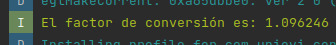
\includegraphics[width=\textwidth]{71/Conversion.jpg}
	\captionof{figure}{Ratio de EUR a USD}\label{fig:71/1}
\end{minipage}

A continuación, se muestra una captura de pantalla de la interfaz de usuario tras
haber realizado un cambio de euros a dólares:

\begin{minipage}{\linewidth}
	\centering
	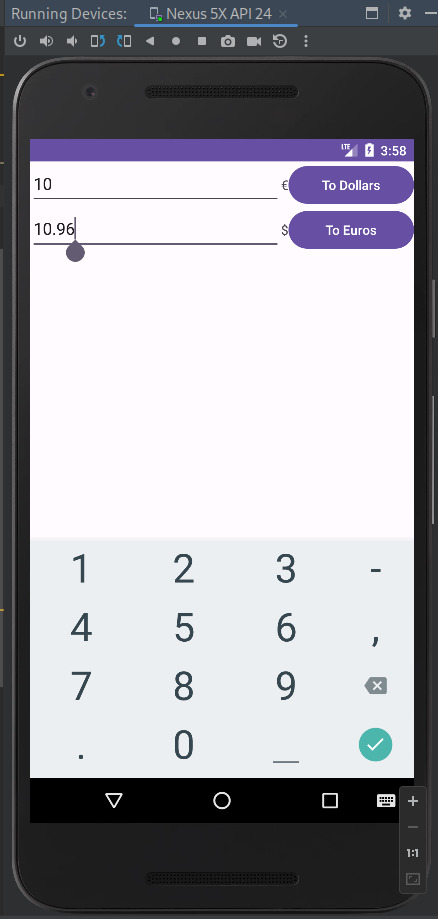
\includegraphics[width=0.4\textwidth]{71/App.jpg}
	\captionof{figure}{Aplicación}\label{fig:71/1}
\end{minipage}

\section{Integración de servicios sobre móviles}\label{sec:7/2}

\subsection{Pintar amigos en el mapa}

\subsection{Integración de serivcios web}

\subsection{Actualización de la posición en función del GPS}

\subsection{Servicios de notificaciones}
